\documentclass[11pt]{article}

\usepackage[catalan]{babel}
\usepackage{translations}
\usepackage[titles]{tocloft}
\usepackage{epigraph} 
\usepackage{multicol}
\usepackage{graphicx} 
\usepackage{amsmath, nccmath}
\usepackage{hyperref}
\usepackage{amsmath}
\usepackage{listings}
\usepackage{courier}
\usepackage[margin=1in]{geometry}
\usepackage{changepage}
\usepackage{titlesec}
\usepackage{wrapfig}
\usepackage[version=4]{mhchem}
\usepackage{multirow}
\usepackage{siunitx}
\usepackage{ragged2e}
\usepackage{adjustbox}
\usepackage[font=small,labelfont=bf]{caption}
\usepackage[table,xcdraw]{xcolor}
\usepackage{afterpage}
\usepackage{xfrac}
\usepackage{animate}

\newcommand{\centered}[1]{\begin{tabular}{l} #1 \end{tabular}}
\newcommand\upvec[1]{\!\vec{\,\mathrm{#1}}}

\definecolor{codegreen}{rgb}{0,0.6,0}
\definecolor{codegray}{rgb}{0.5,0.5,0.5}
\definecolor{codepurple}{rgb}{0.58,0,0.82}
\definecolor{backcolour}{rgb}{0.95,0.95,0.92}

\lstdefinestyle{mystyle}{
    backgroundcolor=\color{backcolour},   
    commentstyle=\color{codegreen},
    keywordstyle=\color{magenta},
    numberstyle=\tiny\color{codegray},
    stringstyle=\color{codepurple},
    basicstyle=\ttfamily\footnotesize,
    breakatwhitespace=false,         
    captionpos=b,                    
    keepspaces=true,                 
    numbers=left,                    
    numbersep=5pt,                  
    showspaces=false,                
    showstringspaces=false,
    showtabs=false,                  
    tabsize=2
}
\lstset{language=Python, 
        basicstyle=\ttfamily\small, 
        keywordstyle=\color{keywords},
        commentstyle=\color{comments},
        stringstyle=\color{red},
        showstringspaces=false,
        identifierstyle=\color{codepurple},
        keywords=[2]{pow},
        keywordstyle=[2]{\color{orange}},
}

\lstset{style=mystyle}
\setlength\parindent{0pt}
\renewcommand{\labelenumi}{\alph{enumi}.}

\setlength\parindent{0pt} % Removes all indentation from paragraphs

\renewcommand{\labelenumi}{\alph{enumi}.} % Make numbering in the enumerate environment by letter rather than number (e.g. section 6)
   
\newcommand{\titulo}{Roda de\\Maxwell\vspace{0.5cm}\\(E2)}
\newcommand{\nombreestudiante}{Víctor Mira Ramírez}
\newcommand{\nombredirector}{Ángel Ávila Freire}
\newcommand{\fecha}{\date{Maig 2023}}  % Definir solo el año de presentación

\pagebreak

\renewcommand{\listtablename}{Índex de taules} 
\renewcommand{\tablename}{Tabla} 
\renewcommand\cftsecdotsep{\cftdotsep}

\setlength{\cftbeforesecskip}{0.5ex}
\renewcommand{\cftsecfont}{%
  \fontsize{11}{13}\usefont{OT1}{phv}{bc}{n}\selectfont
}
\makeatletter
\renewcommand{\@pnumwidth}{1.75em}
\renewcommand{\@tocrmarg}{2.75em}
\makeatother

\begin{document}

\begin{titlepage}
	\centering
	
\includegraphics[width=65mm]{fotos/logoUA.png}\par
	\vspace{1cm}
	{\huge\bfseries \vspace{15mm} \titulo \par}
	\vfill
	{\large 
	\vfill
	Estudiant:\par\vspace{2mm}
	\nombreestudiante\par
	\vfill
	Professor:\par\vspace{2mm}
    \nombredirector
    \vfill
    Universitat d'Alacant\par
    Facultat de Ciències: Departament de Física Aplicada\par
    Tècniques experimentals I\par
	\fecha\par}
\end{titlepage}

\pagebreak

\begin{abstract}\label{sec:abstract}
    \noindent L'objectiu de la pràctica es estudiar les equacions del moviment dinàmic d'un sòlid rígid així com les de conservació de l'energia mecànica mitjançant l'anàlisi del moviment de la Roda de Maxwell. Mesurarem l'acceleració així com el moment d'inèrcia de la roda.
\end{abstract}

\vspace{0.3cm}
\tableofcontents
\newpage

\section{Introducció i motivació}
    Els objectius de la pràctica son els ja descrits a l'\textit{Abstract}, determinar les equacions d'un sòlid rígid mitjançant l'estudi de la \textit{Roda de Maxwell}.  

    \vspace{0.5cm}En física, sovint considerem els cosos com a masses puntuals ja que simplifiquen els problemes àmpliament. Però la realitat no és discreta, milions de partícules formen els cosos amb els que interaccionem diàriament. El cas més simple és el del sòlid rígid. La primera pregunta que se'ns ve al cap és què es un sòlid rígid.

    \vspace{0.5cm}Un sòlid rígid és un cos format per una distribució de masses puntuals equidistants que presenten forces de cohesió que es suposen tan fortes que el cos es indeformable. Destaquem que es tracta també d'una idealització per a resoldre problemes un una massa puntual s'allunya massa (valgui la redundància) de la realitat.

    \vspace{0.5cm}A l'experiment considerem la \textit{Roda de Maxwell} com a un sòlid rígid continu, es a dir, que les partícules que composen el sòlid son infinites i indistingibles. Per a una major profunditat sobre la roda, veure apèndix \ref{appendix:maxwell} i \ref{appendix:roda}.

    \vspace{0.5cm}El moviment d'un sòlid rígid es descompon en translació i rotació, objecte d'estudi a la pràctica. A fi de profunditzar en aquests resultats i aportar conclusions, realitzem aquest breu informe sobre el tema.
    
\section{Marc teòric}
    \subsection{Fonaments de Dinàmica}
        La \textit{Roda de Maxwell} cau en una composició d'un moviment de translació del centre de masses amb un moviment de rotació al voltant de l'eix que passa per el centre de masses.
    
        \begin{wrapfigure}[13]{l}{.3\textwidth}
            \vspace{-1.1cm}
            \begin{center}
                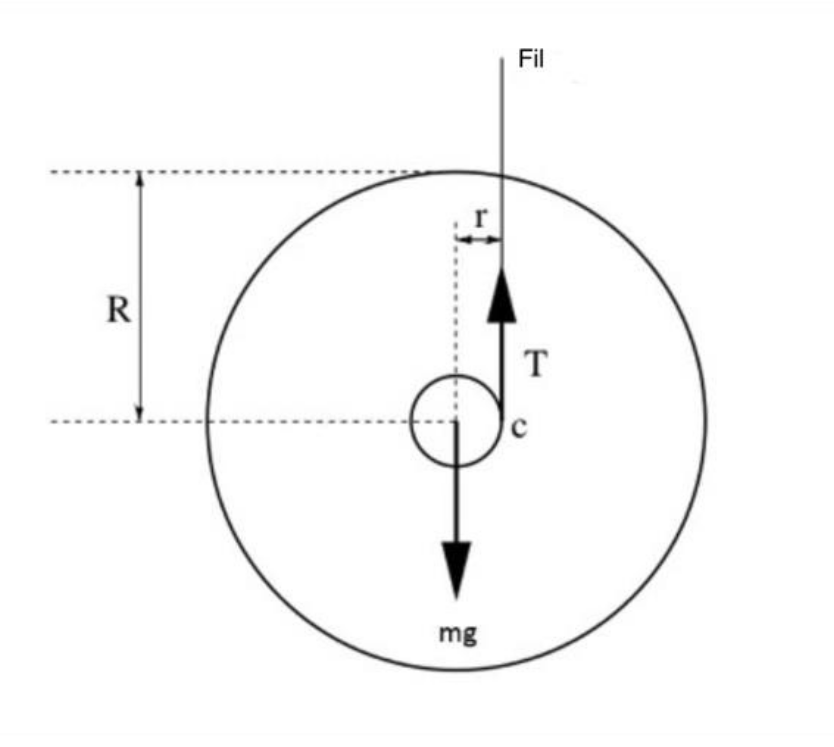
\includegraphics[width=.3\textwidth]{fotos/esquema.png} 
            \end{center}
            \vspace{-0.78cm}
            \caption{Esquema de les forces sobre la \textit{Roda de Maxwell}}
            \label{fig:esquema}
        \end{wrapfigure}
    
        \vspace{0.4cm}La roda girará al voltant del punt c, i l'anomenarem centre de l'eix de rotació. La figura \ref{fig:esquema} és un esquema de les forces que actuen sobre la \textit{Roda de Maxwell} i mostra com les úniques forces que apareixen són el pes de la roda ($mg$) i la tensió del fil ($T$). Anomenarem $R$ al radi de la roda i $r$ al radi de l'eix de rotació.
    
        \vspace{0.4cm}Per a poder descriure el moviment de l'aparell, hem de passar primerament per les equacions fonamentals de la dinàmica. Començant per la \textit{Segona Llei de Newton} (\ref{eq:2newton}), que afirma que \textit{``La força que actua sobre un cos a un instant es proporcional a la variació de moment lineal al mateix instant"}:
    
        \begin{equation}
            \sum \upvec{F}\ =\ \frac{d\vec{p}}{d\vec{t}}
            \label{eq:2newton}
        \end{equation}
    
        \vspace{0.1cm}I coneixent que el moment lineal $p$ es igual a la massa multiplicada per la velocitat $\vec{p}=m\vec{v}$ obtenim:
    
        \begin{equation}
            \sum \upvec{F}\ =\ m\cdot\vec{a}\ =\ \frac{d\vec{p}}{dt}\ =\ \frac{d\left(m\vec{v}\right)}{dt}
            \label{eq:2newton}
        \end{equation}
    
        \vspace{0.1cm}Cal recalcar que aquesta acceleració és la del \textit{cdm} (centre de masses) del dispositiu.
        
    \clearpage
    
        D'altra banda, com la translació i rotació succeeixen a la vegada, podem relacionar fàcilment la velocitat i acceleració lineal amb els seus anàlegs angulars. Recordem també la definició de moment angular.
        \vspace{-0.2cm}
        \begin{equation}
            \vec{v}=\vec{\omega}\cdot\Vec{r}\hspace{1.2cm}\vec{a}=\vec{\alpha}\cdot\vec{r}
            \label{eq:angular}
        \end{equation}
        \begin{equation}
            \vec{L}\ =\ \vec{r}\times\vec{p}\ =\ \vec{r}\times m\cdot\vec{v}
            \label{eq:momAngular}
        \end{equation}
    
        Més concretament per al nostre experiment, coneixem que haurà una variació de $\vec{L}$ respecte al temps, es a dir, el moment angular variarà quan s'aplica sobre el mateix un moment de força.
        \vspace{-0.05cm}
        \begin{equation}
            \frac{d\vec{L}}{dt}\ =\ \frac{d\left(\vec{r}\times\vec{p}\right)}{dt}\ =\ \frac{d\vec{\vec{r}}}{dt}\times\vec{p}+\vec{r}\times\frac{d\vec{p}}{dt}\ =\ \vec{r}\times\vec{F}\ =\ \vec{M}
        \end{equation}
    
        Al tractar-se d'un sòlid rígid com ja hem descrit prèviament, coneixem que $\vec{L}=\vec{I}\times\vec{\omega}$ i per tant, anàlogament a la \textit{Segona Llei de Newton} (\ref{eq:2newton}) obtenim:
        \vspace{-0.05cm}
        \begin{equation}
            \vec{M}\ =\ \frac{d\vec{L}}{dt}\ =\ \frac{d\left(I\cdot\vec{\omega}\right)}{dt}\ =\ I\cdot\vec{\alpha}
        \end{equation}
    
        On el moment d'inèrcia ($I$) soles depèn de la massa i geometria del sòlid rígid i és $I=\int r^2 dm$.
    
        \vspace{1cm}Ara, desenvoluparem el sumatoris de les forces i moments que actuen sobre el \textit{cdm} del cos. 
    
        \begin{equation}
            \begin{cases}\begin{aligned}
                  & \sum\vec{F}\ =\ mg  -   T\ =\ ma\\
                  & \sum\vec{M}_{\textit{cdm}}\ =\ r\times T\ =\ rT\ =\ \alpha I_{\textit{cdm}}\\
            \end{aligned}\end{cases}
            \label{eq:sumatorios}
        \end{equation}
    
        Coneixent i desenvolupant \ref{eq:angular} arribem a que $\alpha=\frac{a}{r}$, que ens deixa el sistema d'equacions com:
    
        \begin{equation*}
            \begin{cases}
                mg-T=ma\\
                rT=I\mfrac{a}{r}\\            
            \end{cases}
            \hspace{-0.3cm}\Longleftrightarrow
            \begin{cases}
                a=g-\mfrac{T}{m}\\
                T=I\mfrac{a}{r^2}\\            
            \end{cases}
            \hspace{-0.2cm}\Longleftrightarrow
            \ a+\frac{Ia}{r^2m}=g\ \Longleftrightarrow\ a\left(1+\frac{I}{r^2m}\right)=g\ \Longleftrightarrow
        \end{equation*}
    
        \begin{equation}
            \begin{tabular}{ @{}c@{} @{}c@{} }
                \centered{$\boxed{a=\frac{g}{1+\mfrac{I}{r^2 m}}}$} & \centered{$\boxed{I=\left(\frac{g}{a}-1\right)r^2m}$}\\
            \end{tabular}
            \label{eq:acceleracio}
        \end{equation}
    
        I obtenim a \ref{eq:acceleracio} una expressió pera l'acceleració. Observem com aquesta és constant i soles depèn de $g$, l'acceleració gravitatòria, i de $m$ i $r$, que són propietats intrínseques del cos. Això ens indica que la roda descriurà un moviment uniformement accelerat (MRUA), que segueix les equacions següents per a la posició ($y(t)$) i la velocitat $v(t)$ en funció del temps:
    
        \begin{equation}
            \begin{cases}
                y(t) = \frac12 at^2\\
                v(t) = at\\
            \end{cases}
            \label{eq:mrua}
        \end{equation}

    \clearpage
    \vspace{-0.4cm}
    \subsection{Conservació de l'energia mecànica}
        Després del degut anàlisi de la dinàmica de la \textit{Roda de Maxwell}, resulta convenient estudiar el moviment descrit pel cos mitjançant energies.

        \vspace{0.3cm}Com deixem caure la roda des d'una altura inicial ($h$), aquesta obtindrà conseqüentment energia potencial gravitatòria ($U_g$). Caient, guanyarà velocitat lineal ($v$) així com velocitat angular ($\omega$), es a dir, la roda canviarà la $U$ administrada per energia cinètica tant de translació ($K_t$) com de rotació ($K_r$) al voltant de l'eix del seu \textit{cdm}. Definim les equacions de les tres energies:

        \vspace{-0.15cm}
        \begin{equation}
            \begin{cases}
                & U_g = mg\cdot h\\
                & K_t = \frac12 mv^2\\
                & K_r = \sum\frac12 m_i v^2_i\ =\ \sum\frac12 m_i r^2_i \omega^2_i\ =\ \frac12 I\omega^2\\
            \end{cases}
        \end{equation}

        Per al cas del treball realitzat per el cos ($W$), podem definir-ho com una variació entre els punts inicial i final d'energia cinètica ($W=\Delta\left(K_t+K_r\right)$) o canviant el signe com una variació d'energia potencial ($W=-\Delta U_g$), però aquest últim solament es cert quan parlem de forces conservatives, com és el cas al nostre experiment. Podem relacionar ambdues expressions i obtindre:
        \vspace{-0.15cm}
        \begin{equation}
            \Delta K=-\Delta U\implies\Delta K + \Delta U = 0 
            \label{eq:potencial}
        \end{equation}

        \vspace{-0.2cm}I així, hem d'incloure les forces de fregament que puguen ocórrer entre el fil i la barra, així com el fregament de l'aire i d'altres interaccions no desitjades que ocorren en la vida real. Nombrarem a aquestes forces com a $W_f$ (treball de fregament). Finalment, obtenim com a expressió per a l'energia mecànica ($E$) en funció del temps la següent equació, tenint en compte la expressió \ref{eq:angular}:
        \vspace{-0.1cm}
        \begin{equation}
            E (t)\ =\ U_g + K_t + K_r\ =\ mg\ h(t) + \frac12\left(m+\frac{I_{\textit{cdm}}}{r^2}\right)v^2(t)
        \end{equation}

        \vspace{-0.2cm}Anomenarem a un camp vectorial $ \vec{F}(x,y,z)$ camp conservatiu quan la circulació del camp al llarg d'una curva siga independent del camí, es a dir, depèn únicament dels punts inicial i final. El camp $\vec{F}$ és conservatiu si existeix un camp escalar que verifique que $\vec{F}=-\nabla V$. Aplicant-ho al camp gravitatori:
        \vspace{-0.25cm}
        \begin{equation}
            W_{A\rightarrow B} = \int_A^B \vec{F}\vec{dr}=- \int_A^B \nabla U = U(A)-U(B)=-\Delta U
        \end{equation}
        
        El treball del camp serà independent de la trajectòria, i, si es tracta d'un camp conservatiu, serà igual a la variació d'energia potencial, com ja hem vist a (\ref{eq:potencial}). Si considerem una partícula que es mou per l'eix x sobre la qual actua una força de fregament $\vec{F}_R=-\mu mg$, podem definir el treball de la força de fregament com a la següent expressió, on $x$ es la distància entre $A$ i $B$.
        \vspace{-0.1cm}
        \begin{equation}
            W_{A\rightarrow B}=\int_A^B\vec{F}_R\ d\vec{r}=-\mu mgx=\int_B^A\vec{F}_R\ d\vec{r}=W_{B\rightarrow A}
        \end{equation}
        
        Quan una força és conservativa, el treball que realitza és independent del camí. Si aquest treball es realitza sobre una curva tancada, el treball total que realitza la força serà zero. Si calculem el treball total dels dos casos que hem vist, obtenim que $W_{total} = W_{A\rightarrow B}+W_{B\rightarrow A}=-2\mu mgx \neq 0$ i per tant la força de fregament no es conservativa ni pot tindre associat cap potencial.
        
        \vspace{0.3cm}Aplicant la \textit{Segona Llei de Newton} (\ref{eq:2newton}) arribem al principi de conservació de la energia mecànica:
        \begin{equation}
            \int_{t_1}^{t_2} \vec{F}\vec{dr} =m\int_{t_1}^{t_2}\frac{dv}{dt}vdt=\int_{t_1}^{t_2}\frac{d}{dt}\left(\frac{1}{2}mv^2\right)dt=\frac{m}{2}(v(t_2)-v(t_1))=K(t_2)-K(t_1)
        \end{equation}
        I igualant els resultats obtinguts:
        \begin{equation}
        \notag U(t_1)-U(t_2)= K(t_2)-K(t_1)\Rightarrow K(t_1)+U(t_1)=K(t_2)+U(t_2)\Rightarrow\boxed{{E(t_1)=E(t_2)}}
        \end{equation}
        Per tant podem concloure que l'energia mecànica es conserva.

        
\clearpage
\section{Procediment experimental}
    \subsection{Material}
        \begin{multicols}{2}
            \begin{itemize}
                \item \textit{Roda de Maxwell} \ref{appendix:roda}
                \item Regla graduada
                \item Nivell
                \item Peu de rei
                \item Trípode
                \item Balança granetària \ref{appendix:granetaria}
            \end{itemize}
        \end{multicols}
        
        Amb el peu de rei vam mesurar el radi de la \textit{Roda de Maxwell} i amb la balança vam mesurar la seua massa. El trípode va ser utilitzat per a col·locar un telèfon mòbil que farà de càmera de vídeo. Per a després poder analitzar el vídeo per a obtindre dades de temps i posició, hem d'assegurar-nos de calibrar una regla graduada al costat de la disposició experimental. Amb l'objectiu de col·locar horitzontalment la taula on disposarem la \textit{Roda de Maxwell} farem ús d'un nivell.

        \vspace{0.4cm}Després de realitzar mesures amb el peu de rei del diàmetre de l'eix de rotació a punts diferents: 5.1, 5.0 i 5.1 $\pm$ 0.1 mil·límetres, obtenim (després del tractament estadístic i de l'error) un valor per al radi de: $r = 5.1 \pm 0.1$mm. De la mateixa manera vam realitzar diverses mesures de la massa de la roda mitjançant la balança granetària i vam obtindre un valor final de $m = 510.4\pm0.1\si{\gram}$. Per a obtindre les dades del vídeo experimental, utilitzarem el programa \textit{Tracker}, un programa de tractament de vídeo. Per a l'anàlisi de les dades i la realització de gràfiques utilitzarem el llenguatge de programació python juntament amb la llibreria de tractament de bases de dades \textit{pandas} i la de impressió de gràfiques \textit{matplotlib}.

        \begin{figure}[h]
            \label{fig:disposicio}
            \vspace{-0.4cm}
            \begin{center}
                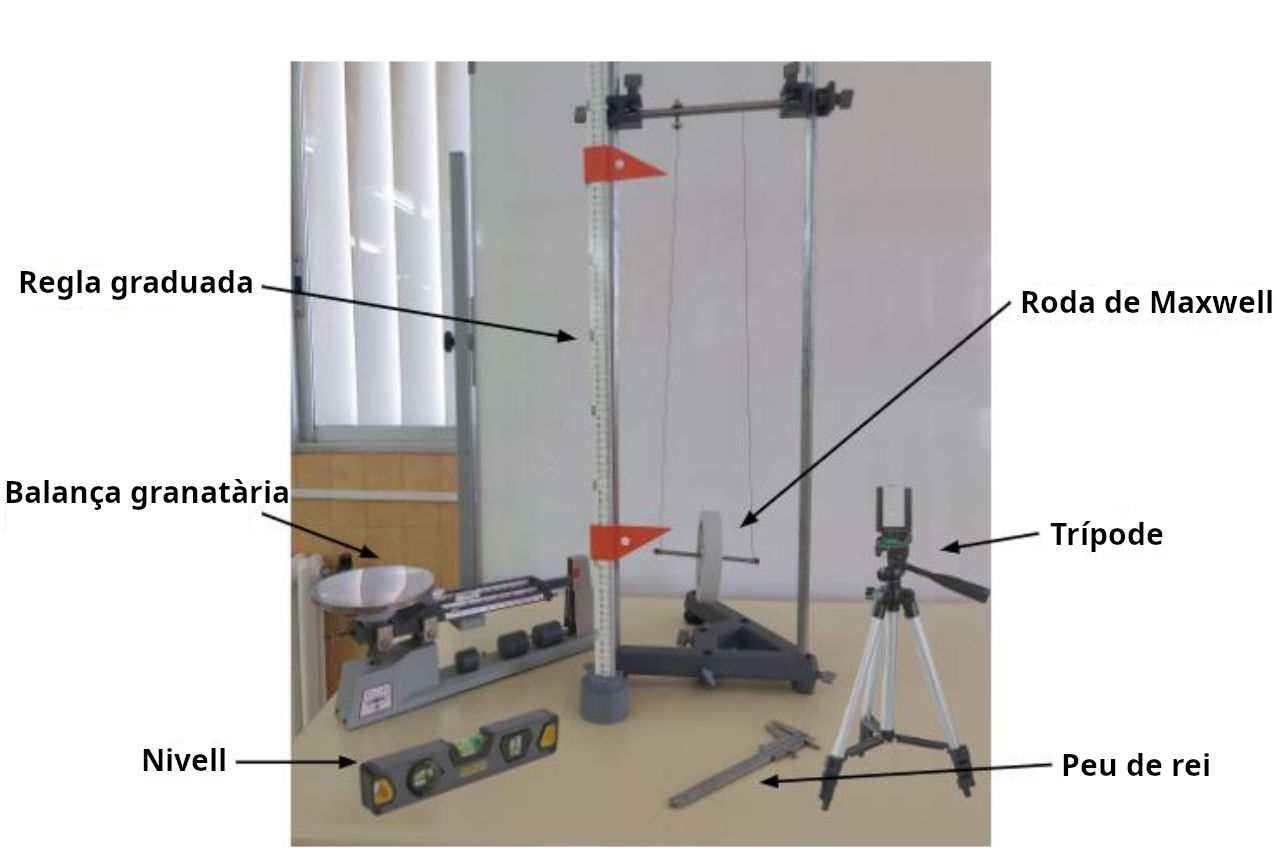
\includegraphics[width=.62\textwidth]{fotos/disposicio.png}
                \caption{Disposició experimental}
            \end{center}
        \end{figure}
        \begin{figure}[h]
            \begin{center}
                
\includegraphics[width=.22\textwidth]{fotos/tracker.png}
                
\includegraphics[width=.22\textwidth]{fotos/matplotlib.png}
            \end{center}
        \end{figure}
        
    \subsection{Metodologia} 
        Primerament, com ja hem detallat a l'apartat anterior, tractarem de anivellar el dispositiu experimental, amb cura de que la roda estiga paral·lela a la taula. Una vegada hem col·locat la càmera a una distància sensata, hem de calibrar la càmera. I es que el programa que utilitzem per a treure dades del vídeo, \textit{tracker}, funciona comparant el contrast de píxels amb els confrontants. \textit{Tracker} té una funció anomenada \textit{autotracker} que busca automàticament un punt del vídeo als fotogrames següents, permetent-nos extreure les dades amb un clic. Podem veure una captura de pantalla del programa a la figura \ref{fig:autotracker}.

        \begin{wrapfigure}[14]{r}{.48\textwidth}
            \vspace{-0.35cm}
            \caption{\textit{Autotracker}}
            \vspace{-0.5cm}
            \begin{center}
                \label{fig:autotracker}
                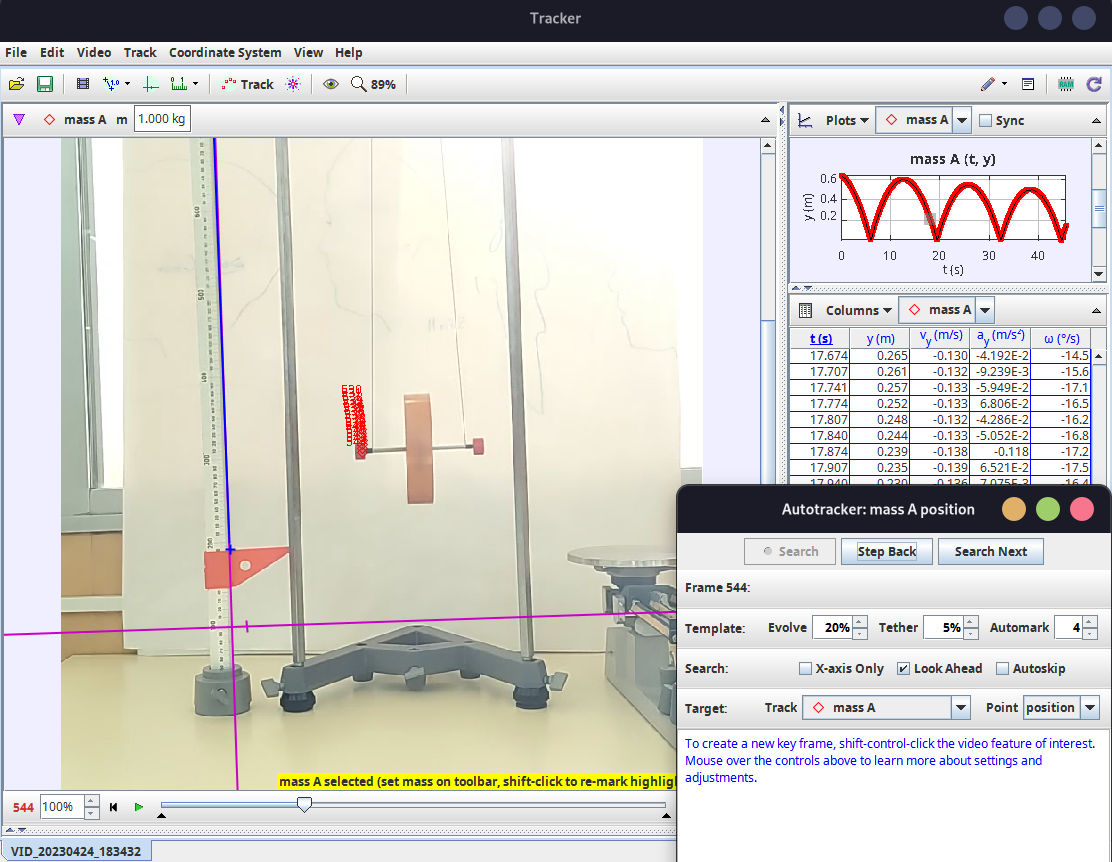
\includegraphics[width=.48\textwidth]{fotos/autotracker.png}
            \end{center}
        \end{wrapfigure}
        
        \vspace{0.4cm}Per a facilitar que el programa funcione automàticament i no haguem d'introduir cap punt manualment, augmentarem la exposició de la càmera dràsticament.  Tot i que el vídeo es vorà massa clar i amb aparença llavada, aconseguirem que tot el fons que envolta la roda siga completament blanc, facilitant el treball a \textit{autotracker}.

        \vspace{0.4cm}L'augment d'exposició va ajudar-nos amb altres dificultats que vam trobar originalment als vídeos, un efecte anomenat \textit{banding}. L'efecte, que es produeix quan la freqüència del sensor de la càmera coincideix amb la freqüència d'una fons de llum. Al nostre cas, el laboratori era il·luminat per tubs incandescents, que tenen una freqüència de $60\ \si{\hertz}$, i al coincidir amb els \textit{fps} o \textit{frames per second} estàndard (fotogrames per segon) a una càmera de vídeo, $60$ \textit{fps}, produïa l'efecte no desitjat.

        \vspace{0.4cm}Augmentar l'exposició, així com canviar els \textit{fps} a $90$, ens va permetre eliminar l'efecte de \textit{banding} i obtindre una major densitat de dades com a conseqüència ja que tenim més fotogrames per segon i per tant més resolució.

        \begin{figure}[h]
            \begin{center}
                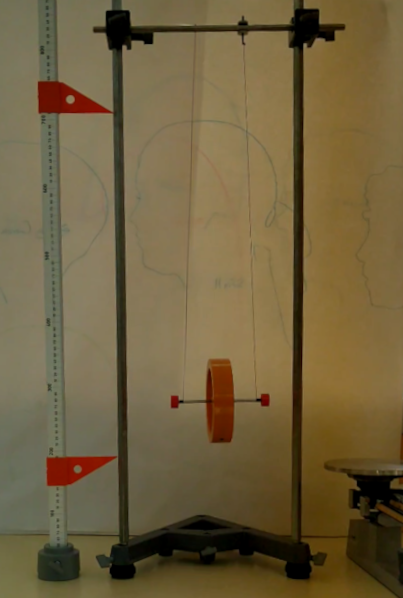
\includegraphics[width=.21\textwidth]{fotos/banding1.png}
                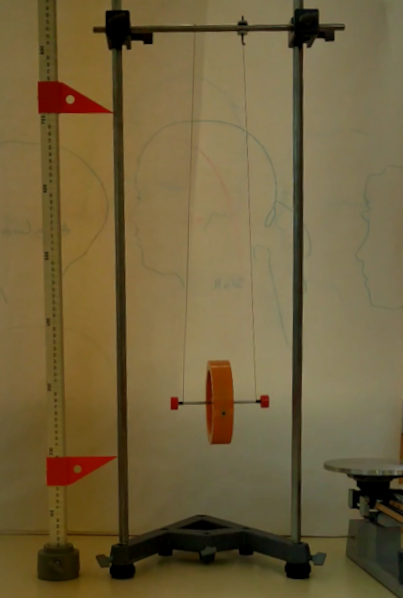
\includegraphics[width=.21\textwidth]{fotos/banding2.png}
                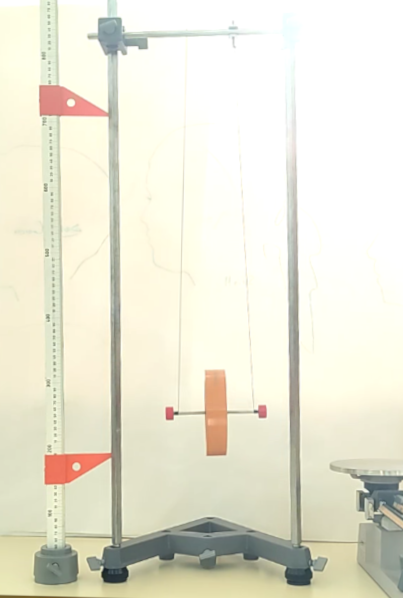
\includegraphics[width=.21\textwidth]{fotos/banding3.png}
            \end{center}
            \vspace{-0.5cm}
            \caption{Dos fotogrames amb \textit{banding} i un fotograma amb exposició augmentada}
        \end{figure}

        A la figures podem observar clarament com als dos primers fotogrames apareixen bandes obscures, a la primera foto trobem una banda a la dreta de la imatge i a la foto d'enmig una banda a l'esquerra de la imatge. Observem com a la última foto no n'hi ha cap banda obscura i, a més, el contrast de la roda amb el fons és molt més ample.
        \clearpage

        Pel que fa al disc, hem d'assegurar-nos de que el fil té la mateixa tensió als dos extrems de l'eix de la roda. Abans de començar a gravar, farem una tirada de prova per comprovar que el fil s'enrola d'una manera compacta i uniforme a ambdós extrems. 

        \vspace{0.4cm}Hem de col·locar una regla graduada al costat de la roda per tal de calibrar les distàncies una vegada a \textit{tracker}. L'altura des de la qual deixem caure la roda no afectarà els càlculs finals, però és recomanable utilitzar una altura sensata: suficientment gran per a tindre dades estables, però sense introduir vibracions a l'eix horitzontal.

        \vspace{0.4cm}Una vegada tenim el vídeo analitzat per \textit{autotracker}, exportarem les dades a un arxiu \textit{.xls} que utilitzarem com a base de dades. Per a llegir les dades a \textit{python} podem utilitzar la llibreria especialitzada \textit{pandas} o bé \textit{xlrd}, amb la qual podrem generar llistes de nombres que \textit{matplotlib} podrà utilitzar per a generar gràfiques. El codi que genera les gràfiques es troba a l'apèndix \ref{appendix:codigo}.

\section{Resultats i discussió}
    \vspace{0.2cm}
    Ara, anem a mostrar els resultats obtinguts a l'experiment, començant amb una representació gràfica de la posició, la velocitat i l'acceleració en funció del temps. Cal dir que vam tomar com a punt de referència el punt més baix de la trajectòria, vam deixar caure la roda completament i allà vam col·locar l'origen.\\
    \begin{figure}[h]
        \vspace{-0.2cm}
        \begin{center}
            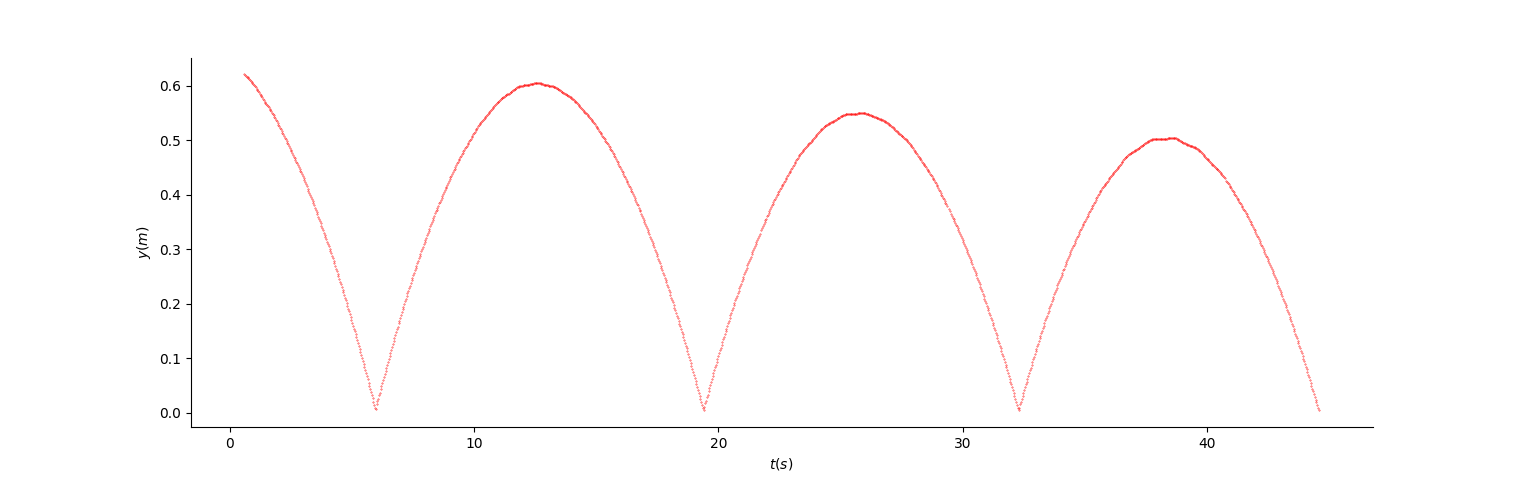
\includegraphics[width=\textwidth]{fotos/posicio.png}
            \caption{Posició, velocitat i acceleració en funció del teps}
        \end{center}
    \end{figure}

    \subsection{Estudi de l'acceleració}
    \vspace{0.4cm}Ara, passem a calcular l'acceleració del \textit{cdm} mitjançant dos mètodes. 
    
    \vspace{0.4cm}El primer, es basa en representar cada bot per separat i ajustar polinomialment la trajectòria parabòlica. L'acceleració l'obtindrem de la meitat del terme quadràtic de l'ajustament, ($mx^2+nx+p$), es a dir, $a=2m$. 

    \clearpage
    
    Tot i que l'aproximació quadràtica és l'aproximació correcta ja que els valors de $R^2$ són pròxims a 1, no s'apropen massa en alguns cassos.

    \begin{figure}[h]
        \vspace{-0.2cm}
        \begin{center}
            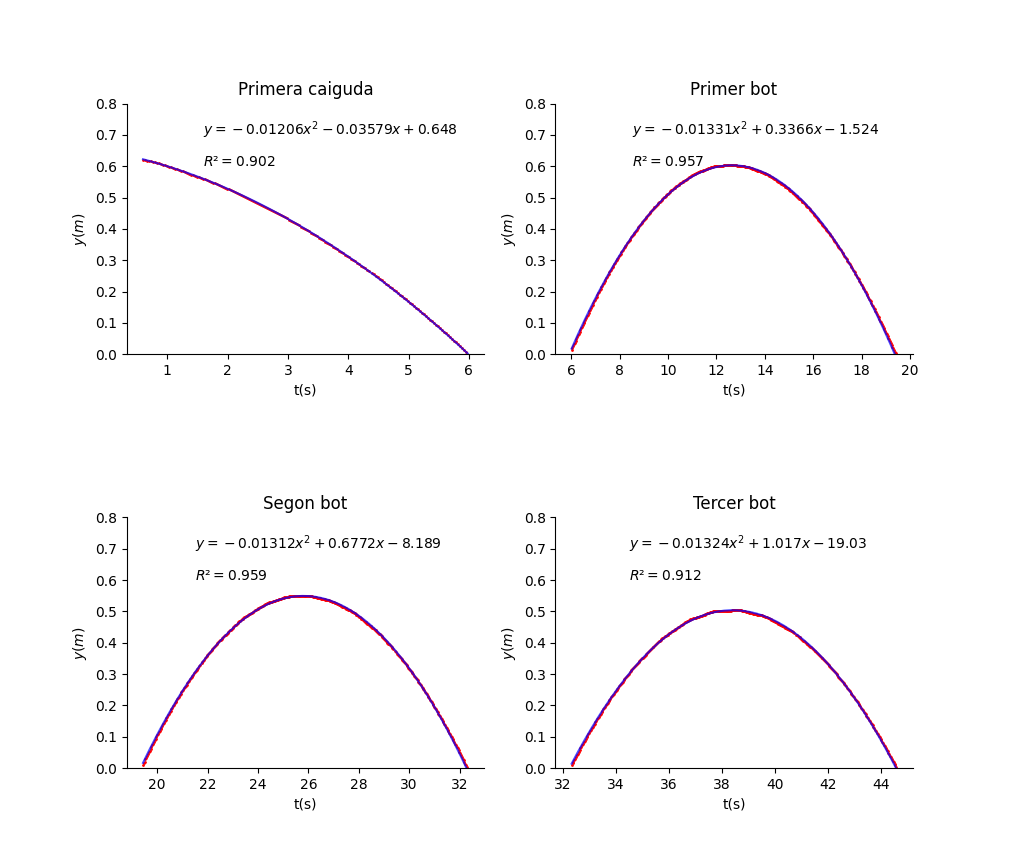
\includegraphics[width=0.8\textwidth]{fotos/4graph.png}
            \label{fig:4graf}
            \caption{Ajustament quadràtic de la posició a cada bot}
        \end{center}
    \end{figure}

    \vspace{0.4cm}A la següent taula trobem les acceleracions calculades per a cada bot, així com el seu error corresponent. El càlcul dels mateixos es detalla a l'apèndix \ref{appendix:errors}
    
    \begin{table}[h]
        \centering
        \begin{tabular}{ccc}
            \rowcolor[HTML]{CBCEFB} 
            \textbf{Bot}                    & \textbf{Terme m}    & \textbf{Acceleració ($m/s^2$)}             \\
            \cellcolor[HTML]{ECF4FF}$0$       & $-0.01206$          & $-0.024 \pm 0.002$\\
            \rowcolor[HTML]{EFEFEF} 
            \cellcolor[HTML]{DAE8FC}$1$       & $-0.01331$          & $-0.027 \pm 0.002$\\
            \cellcolor[HTML]{ECF4FF}$2$       & $-0.01312$          & $-0.027 \pm 0.002$\\
            \rowcolor[HTML]{EFEFEF} 
            \cellcolor[HTML]{DAE8FC}$3$       & $-0.01324$          & $-0.027 \pm 0.002$\\
            \rowcolor[HTML]{FFFFC7} 
            \cellcolor[HTML]{FFFFC7}MITJANA   &$-0.01293$           & $-0.026 \pm 0.002$\\
        \end{tabular}
        \label{tab:acc1}
        \caption{Acceleració mitjançant ajustaments quadràtics de la posició}
    \end{table}

    Finalment, mitjançant el primer mètode, obtenim experimentalment un valor per a l'acceleració lineal de: $$\boxed{a_0=(-0.026\pm0.002)\ m/s^2}$$
    \clearpage

    Continuant amb el segon mètode, estudiarem la representació gràfica de cada bot gràcies a la relació que manté amb la velocitat lineal (\ref{eq:mrua}). La pendent serà l'acceleració en cada bot.

    \begin{figure}[h]
        \vspace{-0.2cm}
        \begin{center}
            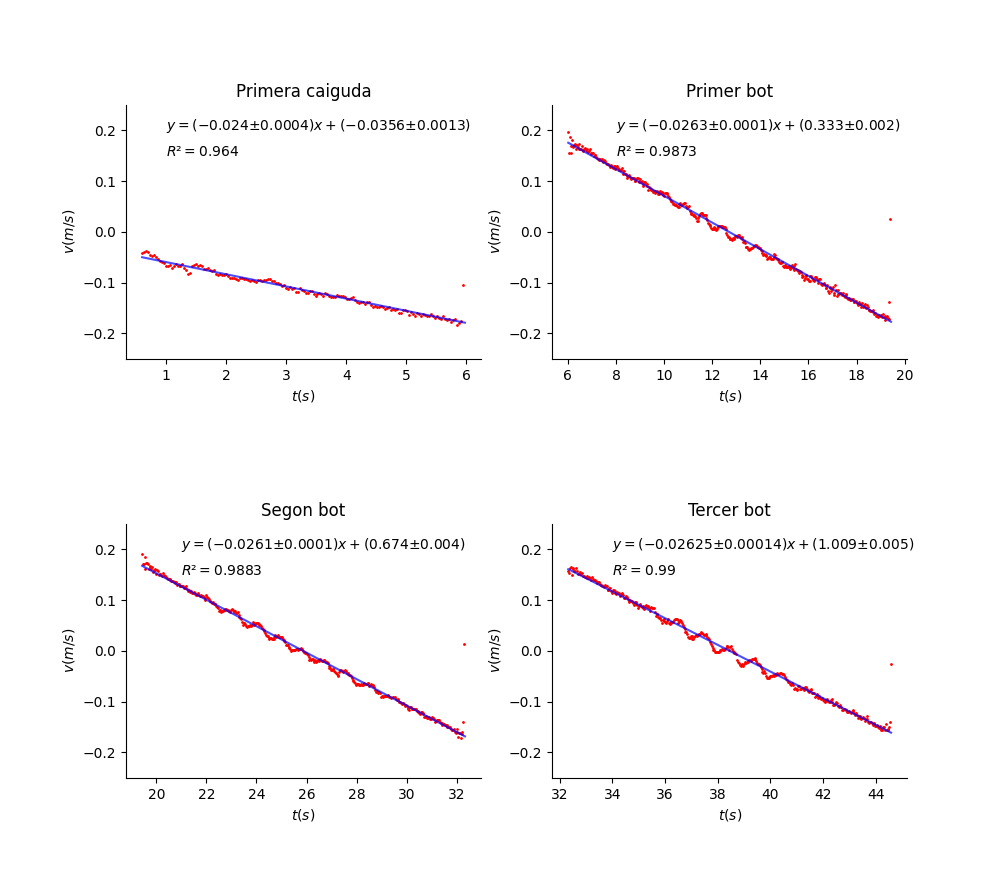
\includegraphics[width=0.8\textwidth]{fotos/velocitat.png}
            \label{fig:4graf}
            \caption{Ajustament lineal de la velocitat a cada bot}
        \end{center}
    \end{figure}

    \vspace{0.4cm}A la següent taula trobem les acceleracions calculades per a cada bot, així com el seu error corresponent. El càlcul dels mateixos es detalla a l'apèndix \ref{appendix:errors}

    \begin{table}[h]
        \centering
        \begin{tabular}{cc}
            \rowcolor[HTML]{CBCEFB} 
            \textbf{Bot}                   & \textbf{Acceleració ($m/s^2$)}                 \\
            \cellcolor[HTML]{ECF4FF}0      & $-0.024 \pm 0.0004$                            \\
            \rowcolor[HTML]{DAE8FC} 
            1                              & \cellcolor[HTML]{EFEFEF}$-0.0263 \pm 0.0001$   \\
            \cellcolor[HTML]{ECF4FF}2      & $-0.0261 \pm 0.0001$                           \\
            \rowcolor[HTML]{DAE8FC} 
            3                              & \cellcolor[HTML]{EFEFEF}$-0.02625 \pm 0.00014$ \\
            \rowcolor[HTML]{FFFFC7} 
            {\color[HTML]{000000} MITJANA} & {\color[HTML]{000000} $-0.0257 \pm 0.0002$}   
        \end{tabular}
        \label{tab:acc2}
        \caption{Acceleració mitjançant ajustaments lineals de la velocitat}
    \end{table}

    Finalment, mitjançant el segon mètode, obtenim experimentalment un valor per a l'acceleració lineal de: $$\boxed{a_1=(-0.0257\pm0.0002)\ m/s^2}$$

    Observem com clarament $a_1$ és una dada més precisa ja que té un error més menut. D'ací en davant aquest serà el valor de l'acceleració que utilitzarem a la resta de l'informe.
    \clearpage

    Calculem ara el moment d'inèrcia per a la acceleració $a_1$ mitjançant la equació (\ref{eq:acceleracio}). El càlcul de l'error es detalla a l'apèndix corresponent \ref{appendix:errors}. $I=(5.052\pm0.013)\cdot 10^{-3}\si{\kilogram}\cdot\si{\meter}^2$

    \vspace{0.4cm}Un mètode alternatiu per a calcular l'acceleració mitjançant les dades de la posició es tomar logaritmes. La caiguda de la roda és descrita per (\ref{eq:mrua}) $y(t) = \frac12at^2$. Tomant logaritmes:

    \begin{equation}
        log(y)=log(\frac{a}{2})+2log(t)
    \end{equation}
    
    La pendent d'aquesta linealització no ens dona cap informació ja que és sempre constant (2). Tot i això, és fàcil comprovar que l'ordenada a l'origen d'aquesta representació és l'acceleració. Després de tindre l'acceleració podem obtindre fàcilment el moment d'inèrcia fent ús de l'equació \ref{eq:acceleracio}. Podem veure la representació a la següent figura.

    \begin{figure}[h]
        \vspace{-0.2cm}
        \begin{center}
            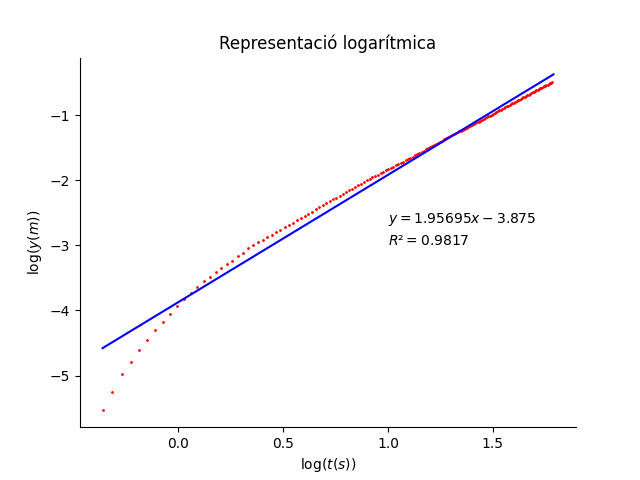
\includegraphics[width=0.8\textwidth]{fotos/log.png}
            \label{fig:log}
            \caption{Energia potencial gravitatòria}
        \end{center}
    \end{figure}

    Obtenint com a recta que linealitza les dades $y = (1.96 \pm 0.02)x + (-3.88 \pm 0.03)$, amb un valor de $R^2 = 0.9817$. L'acceleració serà $2\cdot e$ elevat a l'ordenada a l'origen, és a dir, $a=0.04\pm0.03\ \si{\meter}/\si{\second}^2$. Observem com el valor de la pendent, $1.96$, es pròxim a 2, és a dir, utilitzar una regressió quadràtica per a les dades és una bona aproximació.

    \clearpage
    \subsection{Estudi energètic}
    Anem a fer un estudi energètic del moviment de la roda mitjançant gràfiques de les energies potencial i cinètica, tant de rotació com de translació. Comencem amb la energia potencial:

    \begin{figure}[h]
        \vspace{-0.2cm}
        \begin{center}
            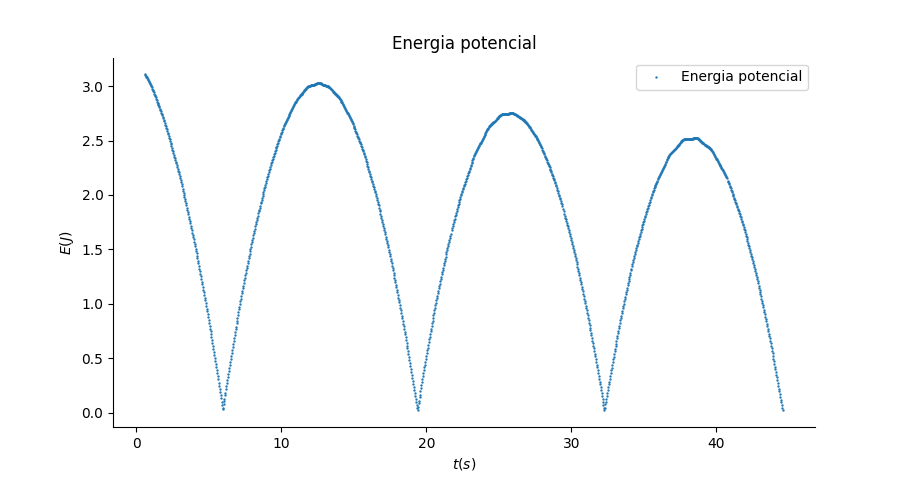
\includegraphics[width=0.8\textwidth]{fotos/energias/u.png}
            \label{fig:u}
            \caption{Energia potencial gravitatòria}
        \end{center}
    \end{figure}

    Observem com inicialment tota la energia del sistema serà potencial i després de cada bot experimenta una caiguda en l'amplitud del pic més alt, degut a les pèrdues energètiques que han ocorregut al llarg de l'experiment.

    \vspace{0.4cm}Grafiquem ara l'energia cinètica, tant de rotació com de translació i observem com la de rotació és molt més significativa. Això ens mostra com quasi tota l'energia potencial es s'empra en fer girar la roda, mentre que una part molt més xicoteta s'empra en pujar i baixar la roda.

    \begin{figure}[h]
        \vspace{-0.2cm}
        \begin{center}
            \begin{tabular}{c c}
                \hspace{-1.15cm}
                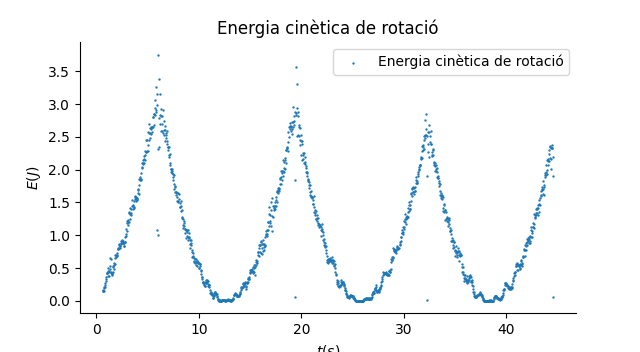
\includegraphics[width=0.55\textwidth]{fotos/energias/kr.png} & 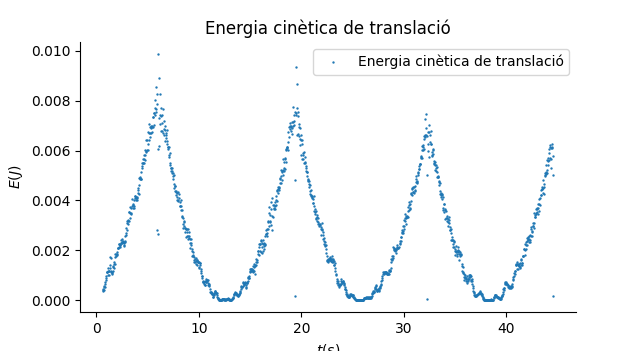
\includegraphics[width=0.55\textwidth]{fotos/energias/kt.png}
            \label{fig:ks}
            \end{tabular}
            \caption{Energia cinètica de rotació i translació}
        \end{center}
    \end{figure}
    \clearpage

    Veiem com clarament la major part de l'energia cinètica és de rotació, ja que els punts de $K_r$ (en taronja) coincideixen amb els de $K$ (en verd) quasi a la perfecció. Recalcar també com els punts de $K_t$ (en blau) són molt pròxims a zero, i es troben 3 ordres de magnitud per davall de el seu anàleg de rotació.
    \begin{figure}[h]
        \vspace{-0.2cm}
        \begin{center}
            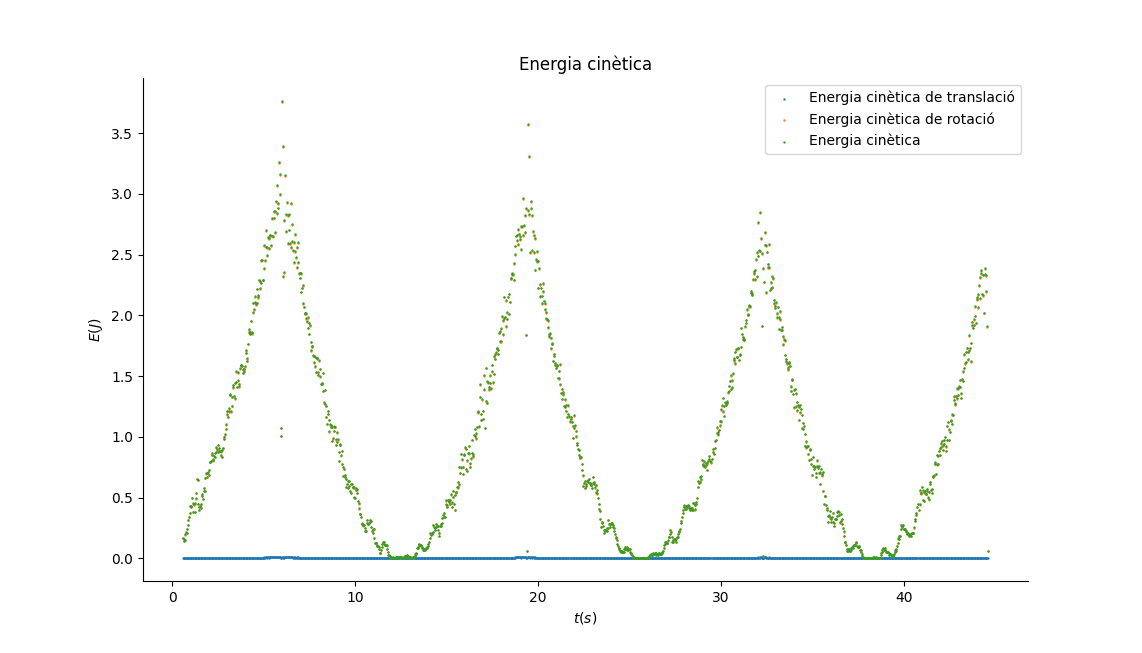
\includegraphics[width=0.8\textwidth]{fotos/energias/k.png}
            \label{fig:k}
            \caption{Energia cinètica}
        \end{center}
    \end{figure}

    \begin{wrapfigure}[16]{l}{.55\textwidth}
        \vspace{-1.2cm}
        \begin{center}
            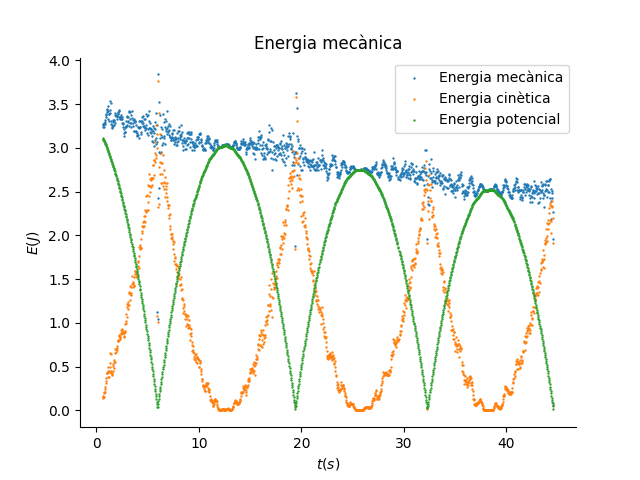
\includegraphics[width=0.6\textwidth]{fotos/energias/e.png}
            \label{fig:e}
            \vspace{-0.2cm}
            \caption{Energia mecànica}
        \end{center}
    \end{wrapfigure}

    Ara, passarem a graficar l'energia mecànica, que no es més que la suma de l'energia cinètica i de l'energia potencial. Observem com decau en funció del temps a causa del treball de les forces no conservatives. Podem concloure que l'energia no es conserva totalment al nostre experiment, per la existència de forces no conservatives com ara el fregament de la roda amb l'aire. Observem com als punts on rebota la roda el programa \textit{tracker} té problemes per a calcular la posició ja que utilitzem un mètode discret per a obtindre les dades. És molt difícil coincidir amb el punt més baix de la trajectòria i sovint introduïm errors d'aquesta manera.
    
\clearpage    
\section{Possibilitats de millora}
    Anem a parlar de possibles millores d'aquest desenvolupament experimental, tot i que els resultats positius mostren que ja es gairebé un bon experiment. Una millor selecció de material sempre ajudarà a la qualitat de la pràctica, des d'una càmera amb major qualitat de post-processat que evite el \textit{banding} experimentat a més de donar la possibilitat de gravar a diferents \textit{fps}, fins a una col-locació de l'experiment lluny de la finestra per a evitar que les càmeres hagen de gravar a la contra de la llum natural del sol. 

    \vspace{0.4cm}Altra possible millora és posar un motor que enrole la roda automàticament, per a així eliminar el factor humà que s'introdueix en la qualitat de l'enrolament del fil a l'eix de la roda.

    \vspace{0.4cm}Agrair la col·laboració del tècnic de laboratori \textit{Samuel Esteve de la Ossa} al laboratori de física aplicada en el desenvolupament d'aquesta pràctica així com totes les anteriors realitzades a \textit{Tècniques Experimentals I}

    
\section{Conclusions}

    A aquest informe es detalla el moviment de un sòlid rígid com és la \textit{roda de Maxwell} des del punt de vista de la dinàmica, així com el principi de conservació de l'energia mecànica a camps vectorials conservatius.
    
    \vspace{0.35cm}El fregament juga un paper important a la vida reial, que produeix que les dades obtingudes mostren la naturalesa no-conservativa del moviment de la roda. Aquest moviment no és més que el moviment d'un yo-yo, el moviment d'un cos en rotació resulta molt interessant per als estudiants del grau en física.

    \vspace{0.35cm}Dominar l'ús de programes de tractament de vídeo com \textit{tracker}, així com de tractament de dades matemàtiques com \textit{python} o de redacció d'informes matemàtics formals com \textit{LaTeX} és altament enriquidor i requereix un domini del camp d'estudi previ a la realització de documents com aquest.

\clearpage
\section{Apèndixs}
    \subsection{James Clerk Maxwell}\label{appendix:maxwell}
        \vspace{0.2cm}
        \begin{wrapfigure}[12]{l}{.26\textwidth}
            \vspace{-0.89cm}
            \begin{center}
                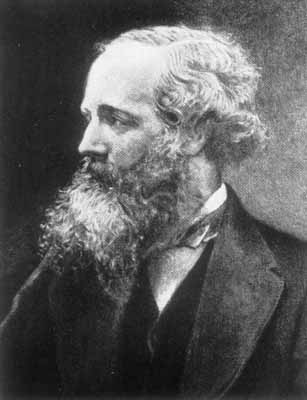
\includegraphics[width=.255\textwidth]{fotos/maxwell.jpeg}
            \end{center}
        \end{wrapfigure}
        \textit{James Clerk Maxwell} (1831-1879) fou un físic teòric i matemàtic escocès. El descobriment més important que va realitzar va ser al camp de l'electromagnetisme, ja que les equacions que porten el seu nom van aconseguir unificar el camp d'estudi. La seua investigació sobre l'electromagnetisme fan d'ell un dels grans científics de la història.\\
        
        El llibre on il·lustra les seues idees va ser \textit{Treatise on Electricity and Magnetism} (o 'Tractat sobre Electricitat i Magnetisme') de 1873. Al text, \textit{Maxwell} tracta les idees de \textit{Michael Faraday} a equacions matemàtiques: es desenvolupa un model matemàtic per a tractar d'explicar la \textit{Llei d'Inducció de Faraday} (un camp magnètic variable pot induir camps electromagnètics). A més es plateja la existència de corrents de desplaçament als dielèctrics i va deduir que les ones electromagnètiques es propaguen transversalment a la velocitat de la llum, $c$. \\

        També va contribuir al camp de la mecànica estadística amb l'anomenat distribució de Maxwell-Boltzmann, una manera de descriure estadísticament la teoria cinètica dels gasos. Va presentar la primera fotografia a color realment duradora i va contribuir al disseny estructural de molts ponts.\\ 

        Els seus descobriments senten les bases de la física moderna com son la relativitat especial o la mecànica quàntica. Es considerat per molts el científic del segle XIX amb més influència al segle XX. I es reflexa a l'enquesta dels millors 100 físics de la història, on va quedar tercer, només rere \textit{Albert Einstein} i \textit{Isaac Newton}.

        \epigraph{"El treball de Maxwell és el més profund i fructífer que la física ha experimentat des de l'època de Newton"}{\textit{Albert Einstein}}

    \vspace{-0.5cm}
    \subsection{Roda de Maxwell}\label{appendix:roda}
        \vspace{0.2cm}
        \begin{wrapfigure}[12]{r}{.26\textwidth}
            \vspace{-1.1cm}
            \begin{center}
                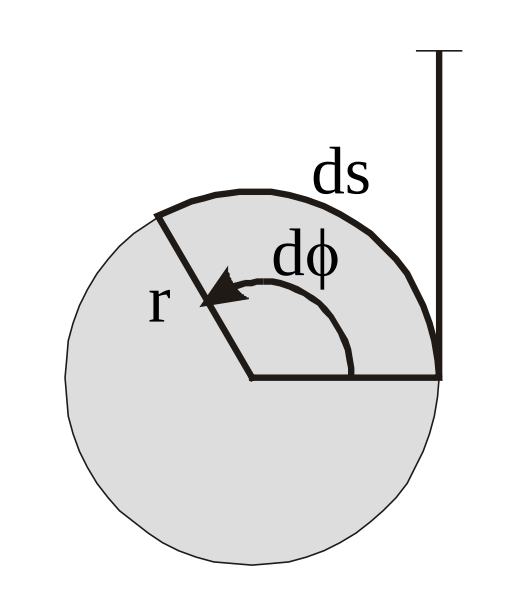
\includegraphics[width=.255\textwidth]{fotos/rueda.png}
            \end{center}
        \end{wrapfigure}
        A aquest apèndix descriurem succintament el dispositiu experimental que s'ha utilitzat al laboratori, la \textit{Roda de Maxwell}. Es tracta d'un aparell molt utilitzat als laboratoris de totes les universitats del mon a fi d'il·lustrar la llei de conservació de l'energia.\\ 

        El dispositiu consta d'una corda enrolada a l'eix d'un disc de massa $m$ i radi $R$. Fixem la corda per un extrem i soltem el disc. Observem com una vegada deixem el disc caure aquest girarà sobre l'eix on la corda està enrolada d'una forma similar a un \textit{"yo-yo"}. Considerem la corda com a inextensible i sense massa.

    %---------------------------------%
    \clearpage
    %---------------------------------%

    \subsection{Balança granetària}\label{appendix:granetaria}
        \vspace{0.2cm}
            \begin{wrapfigure}[5]{r}{.27\textwidth}
                \vspace{-0.85cm}
                \begin{center}
                    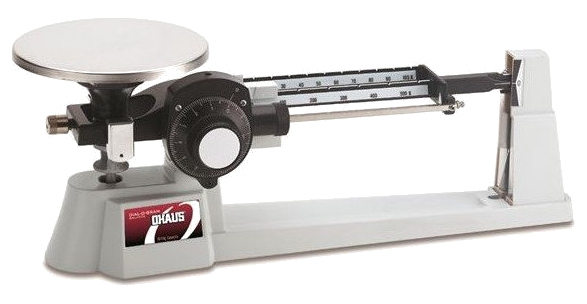
\includegraphics[width=.27\textwidth]{fotos/granataria.png}
                \end{center}
            \end{wrapfigure}
        Una balança granetària es una balança mecànica de precisió que té un rang de mesura entre $200\si{\gram}$ i $25\si{\kilogram}$. Entre els avantatges d'utilitzar una balança d'aquest tipus trobem que requereix un manteniment inferior a altres, a més de que resulta més econòmica. Porta el nom de granetària ja que té tres tipus de barres per a realitzar les mesures de diferents grandàries, que habilita als científics per a determinar analògicament el pes i per tant la massa d'objectes diversos. Les barres tenen la funció de lliscar horitzontalment per a calibrar les mesures. Les barres es desplacen per una biga sòlida fixa a un fulcre i amb un extrem amb un punter i altre acabat en un plat. Al plat depositarem els objectes de mesura.
    
        \vspace{0.5cm}Per a utilitzar la ferramenta, el primer pas es calibrar el instrument. Per a aquesta tasca disposem d'un caragol de tarat que girarem en un sentit o altre fins a que el punter coincidisca amb el 0. Posteriorment, depositarem l'objecte al plat i mourem la barra més gran cap al punter fins a que aquest passe el 0. Utilitzarem la mesura anterior i continuarem amb la següent barra més gran procedint de la mateixa manera. Una vegada totes les barres de la balança han sigut utilitzades i el punter marca el 0, basta sumar la massa de totes les barres per a obtindre una mesura de l'objecte.
    
        \vspace{0.5cm}Encara que els avantatges d'aquesta balança la fan molt bona per a l'ús de laboratori didàctic (és una balança mecànica que manca de elements electrònics i per tant d'un manteniment extensiu) no gaudeix de la precisió d'una balança electrònica. Tot i això, la natura analògica del dispositiu requereix d'higiene ja que qualsevol brutesa que trobem al plat afectarà a la mesura com a qualsevol altra balança.

    \subsection{Càlcul d'errors}\label{appendix:errors}
        El càlcul de l'error del moment d'inèrcia s'obté mitjançant propagació d'errors amb la expressió següent, coneixent que les variables mesurades han sigut $r,m$ i $a$:

        $$\mu\left(I\right)=\sqrt{\left(r^2\left(\frac{g}{a}-1\right)\mu\left(m\right)\right)^2+\left(2rm\left(\frac{g}{a}-1\right)\mu\left(r\right)\right)^2+\left(mr^2\left(\frac{g}{a^2}+1\right)\mu\left(a\right)\right)^2}$$

        \vspace{0.5cm}Per a l'expressió $I=\frac12mr^2$:
        \vspace{-0.3cm}$$\mu\left(I\right)=\sqrt{\left(mr\mu\left(r\right)\right)^2+\left(\frac12r^2\mu\left(m\right)\right)^2}$$

        Per al càlcul de l'error de l'acceleració mitjana així com dels ajustaments polinomials, hem de calcular el desviament típic de la mitjana fent servir:

        \vspace{-0.2cm}
        $$\sigma\left(\vec{a}\right)=\frac{\sigma\left(a\right)}{\sqrt{4}}\text{  on  }\sigma\left(a\right)=\sqrt{\frac{\sum\limits_{i=1}^4\left(a_i-a\right)^2}{3}}$$

        \vspace{0.4cm}Recalcar l'ús del valor estàndard acceptat per a l'acceleració de la gravetat terrestre: $g=9.80665\si{\meter}/\si{\second}^2$
        
    \clearpage
    \subsection{Creació de les gràfiques i de l'informe}\label{appendix:codigo}
        Als següents enllaços es troben el script de \textit{python} que fa les gràfiques que hem vist al llarg de l'informe juntament amb el codi de \textit{LaTeX} que compilat genera este informe.
        \begin{itemize}
            \item \href{https://github.com/vmr48-ua/extras/blob/main/TEC1-MyO1.py}{Enllaç al script de python}
            \item \href{https://www.overleaf.com/read/jpfznpdgtrfc}{Enllaç codi de LaTeX}
        \end{itemize}
    
\section{Referències}   
    \href{https://www.tablesgenerator.com/}{LaTeX tables - tablesgenerator.com}\\

    \href{http://www.upv.es/antenas/Tema_1/james_clerk_maxwell.htm}{James Clerk Maxwell - UPV}\\

    \href{http://www.sc.ehu.es/sbweb/fisica3/solido/maxwell/maxwell.html}{La rueda de Maxwell - sc.ehu.es}\\

    \href{https://ruc.udc.es/dspace/bitstream/handle/2183/16600/LopezDiaz_AnaJesus_2005_Practicas_de_fisica.pdf}{Prácticas de física - ruc.udc.es}\\

    \href{https://physlets.org/tracker/}{Tracker - physlets.org}\\

    \href{https://www.python.org/}{Python3 - python.org}\\

    G. Chiappe, Apuntes mecánica newtoniana y relatividad

\end{document} 